\documentclass{article}

%   Pakete dazuladen
\input{./libs.tex}
%   Farbdefinitionen laden
\input{./colors.tex}
%   \card-Commands laden
\input{./tikzcards.tex}

%   Dummy-Contents
\newcommand{\contentA}{Neunmalkluges Zitat\\mit Bezug zur Karte von einer fiktiven Figur.}
\newcommand{\contentB}{Auswirkungen:\\[5pt]Ziehe 2 Karten, nimm 3 Gold, lege alles ab, lauf weg …}

\begin{document}
\begin{center}
    \pagestyle{empty}
    %   V-Space-Korrektur bei langen Titeln
%   \cardtitle{\vspace{-5mm}SEHR LANGER TITEL}
    \begin{tikzpicture}
        \cardtypeItem
        \cardtitle{Der Schlächter}
        \cardcontent{Sei mein Feind und es ist das Letzte, was du tust.}{\contentB}
        \cardprice{5}
        \cardborder
%       \carddebug
    \end{tikzpicture}
    \hspace{2mm}
    \begin{tikzpicture}
%       \carddebug
        \cardtypeAbility
        \cardtitle{Der Wächter}
        \cardcontent{Keine Sorge, ich mache es lang und äußerst schmerzhaft für dich.}{\contentB}
        \cardprice{35}
        \cardborder
    \end{tikzpicture}
    \hspace{2mm}
    \begin{tikzpicture}
        \cardtypeCharacter
        \cardtitle{Mächtiger Schlächter}
        \cardcontent{Eye, Cäpt'n. Diese Landradd'n werden wir über die Planken schicken!}{\contentB}
        \cardprice{435}
        \cardborder
    \end{tikzpicture}
    \hspace{2mm}
    \begin{tikzpicture}
        \cardtypeTest
        \cardtitle{Schlechter Wächter}
        \cardcontent{Sei Gast in meinem bescheidenen Domizil.}{\contentB}
        \cardprice{$\infty$}
        \cardborder
    \end{tikzpicture}
    \hspace{2mm}
    \begin{tikzpicture}
        \cardtypeItem
        \cardtitle{Schmächtiger Wächter}
        \cardcontent{Miau.}{\contentB}
        \cardprice{5}
        \cardborder
    \end{tikzpicture}
    \hspace{2mm}
    \begin{tikzpicture}
        \cardtypeAbility
        \cardtitle{Gebrechlicher Schlächter}
        \cardcontent{\contentA}{\contentB}
        \cardprice{35}
        \cardborder
    \end{tikzpicture}
    \hspace{2mm}
    \begin{tikzpicture}
        \cardtypeCharacter
        \cardtitle{Gerechter Wächter}
        \cardcontent{\contentA}{\contentB}
        \cardprice{435}
        \cardborder
    \end{tikzpicture}
    \hspace{2mm}
    \begin{tikzpicture}
        \cardtypeTest
        \cardtitle{Welcher Schlächter?}
        \cardcontent{\contentA}{\contentB}
        \cardprice{$\infty$}
        \cardborder
    \end{tikzpicture}
    \hspace{2mm}
    \begin{tikzpicture}
        %\cardbackground{cat.jpg}
        \cardtypeItem
        \cardtitle{Der Schlächter}
        \cardcontent{Sei mein Feind und es ist das Letzte, was du tust.}{\contentB}
        \cardprice{5}
        \cardborder
%       \carddebug
    \end{tikzpicture}
    \hspace{2mm}
    \begin{tikzpicture}
       % \cardbackground{cat.jpg}
%       \carddebug
        \cardtypeAbility
        \cardtitle{Der Wächter}
        \cardcontent{Keine Sorge, ich mache es lang und äußerst schmerzhaft für dich.}{\contentB}
        \cardprice{35}
        \cardborder
    \end{tikzpicture}
    \hspace{2mm}
    \begin{tikzpicture}
       % \cardbackground{cat.jpg}
        \cardtypeCharacter
        \cardtitle{Mächtiger Schlächter}
        \cardcontent{Eye, Cäpt'n. Diese Landradd'n werden wir über die Planken schicken!}{\contentB}
        \cardprice{435}
        \cardborder
    \end{tikzpicture}
    \hspace{2mm}
    \begin{tikzpicture}
       % \cardbackground{cat.jpg}
        \cardtypeTest
        \cardtitle{Schlechter Wächter}
        \cardcontent{Sei Gast in meinem bescheidenen Domizil.}{\contentB}
        \cardprice{$\infty$}
        \cardborder
    \end{tikzpicture}
    \hspace{2mm}
    \begin{tikzpicture}
        \cardtypeItem
        \cardtitle{Schmächtiger Wächter}
        \cardcontent{Miau.}{\contentB}
        \cardprice{5}
        \cardborder
    \end{tikzpicture}
    \hspace{2mm}
    \begin{tikzpicture}
        \cardtypeAbility
        \cardtitle{Gebrechlicher Schlächter}
        \cardcontent{\contentA}{\contentB}
        \cardprice{35}
        \cardborder
    \end{tikzpicture}
    \hspace{2mm}
    \begin{tikzpicture}
        \cardtypeCharacter
        \cardtitle{Gerechter Wächter}
        \cardcontent{\contentA}{\contentB}
        \cardprice{435}
        \cardborder
    \end{tikzpicture}
    \hspace{2mm}
    \begin{tikzpicture}
        \cardtypeTest
        \cardtitle{Welcher Schlächter?}
        \cardcontent{\contentA}{\contentB}
        \cardprice{$\infty$}
        \cardborder
    \end{tikzpicture}
    \hspace{2mm}
     \begin{tikzpicture}
       % \cardbackground{cat.jpg}
        \cardtypeItem
        \cardtitle{Der Schlächter}
        \cardcontent{Sei mein Feind und es ist das Letzte, was du tust.}{\contentB}
        \cardprice{5}
        \cardborder
%       \carddebug
    \end{tikzpicture}
    \hspace{2mm}
    \begin{tikzpicture}
      %  \cardbackground{cat.jpg}
%       \carddebug
        \cardtypeAbility
        \cardtitle{Der Wächter}
        \cardcontent{Keine Sorge, ich mache es lang und äußerst schmerzhaft für dich.}{\contentB}
        \cardprice{35}
        \cardborder
    \end{tikzpicture}
    \hspace{2mm}
    \begin{tikzpicture}
      %  \cardbackground{cat.jpg}
        \cardtypeCharacter
        \cardtitle{Mächtiger Schlächter}
        \cardcontent{Eye, Cäpt'n. Diese Landradd'n werden wir über die Planken schicken!}{\contentB}
        \cardprice{435}
        \cardborder
    \end{tikzpicture}
    \hspace{2mm}
    \begin{tikzpicture}
      %  \cardbackground{cat.jpg}
        \cardtypeTest
        \cardtitle{Schlechter Wächter}
        \cardcontent{Sei Gast in meinem bescheidenen Domizil.}{\contentB}
        \cardprice{$\infty$}
        \cardborder
    \end{tikzpicture}
    \hspace{2mm}
    \begin{tikzpicture}
        \cardtypeItem
        \cardtitle{Schmächtiger Wächter}
        \cardcontent{Miau.}{\contentB}
        \cardprice{5}
        \cardborder
    \end{tikzpicture}
    \hspace{2mm}
    \begin{tikzpicture}
        \cardtypeAbility
        \cardtitle{Gebrechlicher Schlächter}
        \cardcontent{\contentA}{\contentB}
        \cardprice{35}
        \cardborder
    \end{tikzpicture}
    \hspace{2mm}
    \begin{tikzpicture}
        \cardtypeCharacter
        \cardtitle{Gerechter Wächter}
        \cardcontent{\contentA}{\contentB}
        \cardprice{435}
        \cardborder
    \end{tikzpicture}
    \hspace{2mm}
    \begin{tikzpicture}
        \cardtypeTest
        \cardtitle{Welcher Schlächter?}
        \cardcontent{\contentA}{\contentB}
        \cardprice{$\infty$}
        \cardborder
    \end{tikzpicture}
    \hspace{2mm}
    \begin{tikzpicture}
     %   \cardbackground{cat.jpg}
        \cardtypeItem
        \cardtitle{Der Schlächter}
        \cardcontent{Sei mein Feind und es ist das Letzte, was du tust.}{\contentB}
        \cardprice{5}
        \cardborder
%       \carddebug
    \end{tikzpicture}
    \hspace{2mm}
    \begin{tikzpicture}
    %    \cardbackground{cat.jpg}
%       \carddebug
        \cardtypeAbility
        \cardtitle{Der Wächter}
        \cardcontent{Keine Sorge, ich mache es lang und äußerst schmerzhaft für dich.}{\contentB}
        \cardprice{35}
        \cardborder
    \end{tikzpicture}
    \hspace{2mm}
    \begin{tikzpicture}
     %   \cardbackground{cat.jpg}
        \cardtypeCharacter
        \cardtitle{Mächtiger Schlächter}
        \cardcontent{Eye, Cäpt'n. Diese Landradd'n werden wir über die Planken schicken!}{\contentB}
        \cardprice{435}
        \cardborder
    \end{tikzpicture}
    \hspace{2mm}
    \begin{tikzpicture}
     %   \cardbackground{cat.jpg}
        \cardtypeTest
        \cardtitle{Schlechter Wächter}
        \cardcontent{Sei Gast in meinem bescheidenen Domizil.}{\contentB}
        \cardprice{$\infty$}
        \cardborder
    \end{tikzpicture}
    \hspace{2mm}
    \begin{tikzpicture}
        \cardtypeItem
        \cardtitle{Schmächtiger Wächter}
        \cardcontent{Miau.}{\contentB}
        \cardprice{5}
        \cardborder
    \end{tikzpicture}
    \hspace{2mm}
    \begin{tikzpicture}
        \cardtypeAbility
        \cardtitle{Gebrechlicher Schlächter}
        \cardcontent{\contentA}{\contentB}
        \cardprice{35}
        \cardborder
    \end{tikzpicture}
    \hspace{2mm}
    \begin{tikzpicture}
        \cardtypeCharacter
        \cardtitle{Gerechter Wächter}
        \cardcontent{\contentA}{\contentB}
        \cardprice{435}
        \cardborder
    \end{tikzpicture}
    \hspace{2mm}
    \begin{tikzpicture}
        \cardtypeTest
        \cardtitle{Welcher Schlächter?}
        \cardcontent{\contentA}{\contentB}
        \cardprice{$\infty$}
        \cardborder
    \end{tikzpicture}
\end{center}
\end{document}
